\chapter{Product Analysis}

The aim of this chapter is to provide a detailed analysis of the devices more closely related to this project, now that we have a
clearer idea about its main pillars. I will go into many of the available commercial devices and software in the fields of home
automation, voice assistance and smart devices.

\section{Home Automation Systems}
This section covers all the hardware and software systems related to home automation. As we will see, there are lots of solutions
with very different purposes: while there is Amazon Alexa, a full hardware and software system that integrates other home automation
systems, we can also find pure online solutions, like the automation platform IFTTT. Sometimes, home automation systems are
built underneath a virtual assistant, as it happens with Amazon Alexa, so some devices are going to appear in this section and in the
next one. However, they will analyzed from two different perspectives, as having a good virtual assistant does not mean having a
good home automation system.

\subsection{Philips Hue}
Philips Hue is a personal wireless lighting system aimed at the smart home. In combines LED light bulbs, LED strips and other
lighting devices, and sensors that can be configured in their mobile app, so they can modify the home lighting based on a set of
rules. There is a wide range of products, including color and only white lights, so users can build a pretty customizable lighting
experience.\cite{philipsHueMeethue}

The system requires a bridge connected to the Internet (called Philips Hue Smart Hub) in order to work. This is because the Hue
devices do not use WiFi in order to communicate with the bridge, but the system needs to have WiFi to be controllable from a
mobile phone. Thus, it follows a centralized architecture. Moreover, Philips does not provide any type of assistant or external interface
to manage the system apart from the mobile application by default, although Hue works with the most popular home automation
systems, like Alexa or Apple HomeKit, that provide much more flexible home automation management.

\begin{figure}
	\centering
	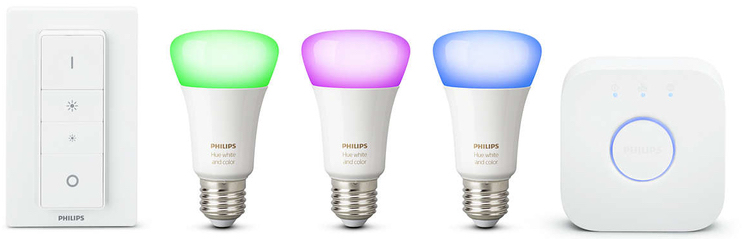
\includegraphics[width=0.9\textwidth]{images/Chapter_04/philips-hue.jpg}
	\caption{A Philips Hue dimmer switch, three color light bulbs and the Hue Smart Hub}
	\label{fig:philips-hue}
\end{figure}

\subsection{LG SmartThinQ}
LG SmartThinQ groups the range of Wi-Fi enabled home appliances made by the company LG, including refrigerators, dishwashers,
vacuum cleaners or air purifiers, between others. As of September 2017, they were the most extensive range of devices of their
kind.\cite{lgSmartThinq}

Unlike Philips Hue, SmartThinQ devices do not require a bridge to work. They can be controlled from the mobile phone and, in some
cases, like in the refrigerators, they include a touchscreen to interact with the device. However, LG does not provide any extra device
or virtual assistant to interact with them, though they are manageable through Amazon Alexa and Google Assistant. A standard setup
with this system will follow a hybrid architecture, as some devices are also their controllers, but there can also be external controllers.

\subsection{Samsung SmartThings}
Samsung SmartThings is a home automation system composed by a series of applications for the Samsung mobile phones, Samsung
TVs and Samung refrigerators. It is even possible to do small management tasks from Samsung smartwatches, called Galaxy Gear. It
uses the cloud to synchronize all the applications, in order to have the most recent information in all of them. This makes it necessary
for the user to have a Samsung account.\cite{samsungSmartthings}

Unlike the previous systems, SmartThings is not a specific system for a range of devices from the same maker, but it is more aimed
to provide an effective interconnection between devices from different makers, as long as they are compatible with their system.
The SmartThings Smart Home Hub is necessary in order to use Samsung SmartThings. It is a bridge that supports common home
automation protocols, like Zigbee or Z-wave, essential to manage some devices that only use these protocols. It also provides
comprehensive automation options.\cite{smartHomeBeginner} The usage of the Hub makes the architecture of this system centralized.

Furthermore, SmartThings is not yet compatible with many commercial devices, and the restrictions imposed by Samsung forces the
user to stick to their environment. In addition, the system is not open source, so making any modification apart from the ones that
Samsung allows is impossible. Also, users are forced to purchase the Smart Home Hub, which makes it necessary to have an additional
device, unlike other similar systems. The system is compatible with Bixby, the virtual assistant from Samsung.

\subsection{Google Home}
Introduced at Google I/O 2016, the annual Google developer conference, \textit{Google Home} is the name of Google's smart speaker,
which is Google's biggest insight into home automation technology. Its aim is to work with all the possible smart home devices, so it
follows the same idea as the Samsung SmartThings system, being a \textit{maker-independent} system, as long as, of course, devices
are compatible with it. Also, Google Home brings all the functions of Google Assistant to the smart speaker.

The main difference with SmartThings is that this system is mainly voice-driven. The home automation layer is pushed down to just
one more function of the virtual assistant, and Google does not even provide a graphical interface to manage the smart devices.
Anyway, normally the makers of each device provide a mobile application from where users can manage their devices in a more
user-friendly interface, but having a centralized view is a desirable feature. On the bright side, all Google devices that support
Google Assistant can automatically control smart home devices.

The number of compatible devices with the Google Assistant, unlike SmartThings, is very high, and almost any new smart home
device is tagged as compatible with it.

\subsection{Apple HomeKit}
HomeKit is the result of Apple's efforts to create a home automation environment adapted to its devices. It has been also made to work
with a wide range of devices, but in this case, Apple included some notable security policies, with the goal of achieving the highest
security and privacy. In fact, all HomeKit devices need to be approved by Apple first.

On iPhone and Mac computers (starting with macOS Mojave), Apple includes an application called Home, which displays all
of the smart home devices in a convenient way and lets people organize and manage them. In addition, it is also possible to establish
automation rules, based on the user's location, time of day, actions or even occupancy of the house. Furthermore, Apple also provides
integration with their personal assistant, Siri. As it happens with the Google Assistant, all Apple devices configured with the same Apple
ID will have the same information automatically synchronized.\cite{appleIOSHome} Usually, systems made under Apple HomeKit will follow
a decentralized architecture.

Although this is a very comprehensive home automation system, the number of compatible devices is not as high as in other options.
Apple has been lately working on promoting their home automation system and their assistant by introducing the HomePod, their smart
speaker with Siri.

\subsection{Somfy}
Somfy is a French company founded in 1960, which since the 1980s has been devoted to the construction of home automation systems.
They have implemented their solutions in important places, like the United Nations Headquarters or the Vancouver Convention Center
and have created their own home automation technologies, such as \textit{Radio Technology Somfy (RTS)} and \textit{Somfy Digital
Network (SDN)}.\cite{somfyOurStory}

Their range of products goes from control devices (as hand-held remotes, mobile applications and wireless switches) and sensors (sunlight,
temperature, wind) to blinds, lighting systems and other smart home utilities. Unfortunately, the control devices only work with Somfy
devices. The system follows a hybrid architecture, where each device is a controller, but there can also be extra controllers, like the
hand-held remotes.
\\~\\

In addition to the previous domotic systems, which are proprietary, there are also open source and more customizable solutions that,
although they may require more time in their configuration, are much more adaptable to the needs of the user. I will explore three of
the most popular: openHAB, Home-Assistant.io and Jeedom.

\subsection{OpenHAB}
OpenHAB, the acronym for Open Home Automation Bus is an open source, technology agnostic home automation platform which runs
as the center of the smart home. \cite{openHABDocs} This means that its aim is to integrate different home automation systems into
a single one. It allows the user to configure almost every aspect of the system, providing a common interface and a uniform approach
to automation rules.

In its most recent version, openHAB 2, it has implemented new user interfaces that automate many processes, so it is almost unnecessary
to write a single line of code, making the system more attractive to all types of users. OpenHAB needs to be installed in a computer that
will act as a server in the local network, making the system accessible via HTTP. It also offers more connectivity options that I will explore
in the following chapters. The architecture, in this case, is decentralized, as there may be multiple controllers, including openHAB itself.

OpenHAB's compatibility is somewhat limited when it comes to home automation devices, but it supports Apple HomeKit and common
protocols, such as ZigBee and Z-Wave, to get rid of specific gateways from other systems.\cite{openHABAddons}

\subsection{Home-Assistant.io}
Home-Assistant.io, or simply Home Assistant, is a open source home automation platform running on Python 3.\cite{homeAssistantio}
Based on a distribution called \textit{Hass.io}, it creates a secured local server in the computer where it is installed. It is accessible via
HTTP and also includes a web user interface that will automate the process of discovering and configuring devices. In terms of
functionality, it is very similar to openHAB, although it might be a little simpler for some users, as it uses the YAML syntax for
configuration, while openHAB has its own.

Its functionality is organized in \textit{Components}, the name that Home Assistant gives to any add-on, which will add a compatibility
layer with a device, system or service. They are fully backed by the Home Assistant community and they are similar in number and type to
what openHAB provides, but with very interesting additions, including Wink and Arduino.

\begin{figure}
	\centering
	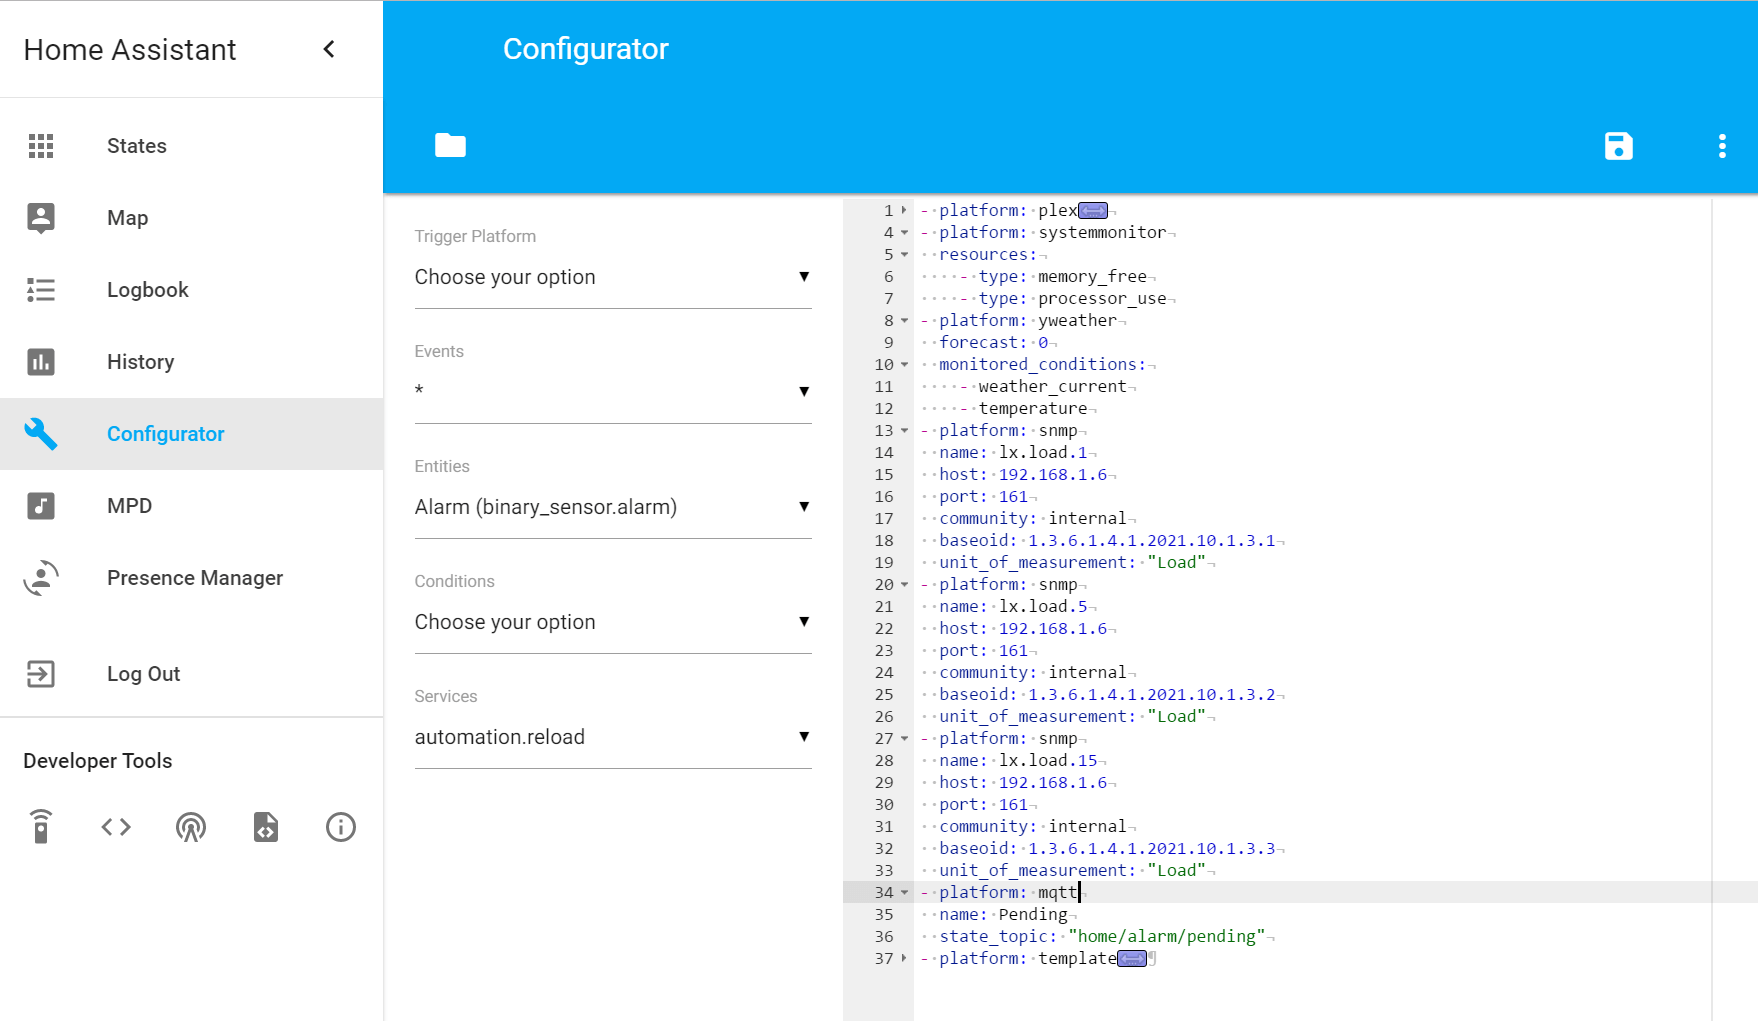
\includegraphics[width=0.95\textwidth]{images/Chapter_04/home-assistant-configuration.png}
	\caption{Home-Assistant.io web user interface}
	\label{fig:home-assistant-configuration}
\end{figure}

\subsection{Jeedom}
Jeedom is a open source, multi-protocol, autonomous and customizable home automation software.\cite{jeedomDoc} It is aimed for
individuals and professionals, and provides custom support for both. They also sell what they call \textit{Boxes}, which are small
computers with Jeedom pre-installed, although their software can be installed on any Linux system. Jeedom also provides mobile phone
apps for Android and iOS, which connect to the Jeedom system by scanning a QR code. As in the previous platforms, they also provide
the \textit{Jeedom Market}, from where users can add new features to their system.

Also, there are different Jeedom versions, which are called \textit{Service packs}. There is the free and open source version, which
includes the lowest number of functionalities. Then, the other versions can be purchased, although some of them come with their Boxes,
and they include dynamic DNS and HTTPS, the mobile application for free or more plugins offered, among other things.

Although the free version is fully open source, the limitations that it has and the obligation to pay in order to have the \textit{full
experience}, could annoy some users and make them lean towards other platforms.
\\~\\

It seems difficult to directly compare these home automation systems, but all of them share characteristics that we can contrast.
The table \ref{table:home-automation-comparison} represents a comparison of the features that I consider most important.

\begin{sidewaystable}[]
	\begin{center}
		\resizebox{\textwidth}{!}{
		\begin{tabular}{|p{0.1\linewidth}|p{0.15\linewidth}|p{0.05\linewidth}|p{0.05\linewidth}|p{0.15\linewidth}|p{0.15\linewidth}|p{0.1\linewidth}|p{0.1\linewidth}|p{0.39\linewidth}|}
			\hline
			\textbf{System name} & \textbf{Developer}                                    & \textbf{Free} & \textbf{Open source} & \textbf{Architecture} & \textbf{Requirements}                               & \textbf{Extra software}                                        & \textbf{Extra hardware}               & \textbf{Compatibility}                                                                                          \\ \hline
			Hue                  & Philips                                               & No                     & No                   & Centralized           & Hue Smart Hub                                       & Mobile app                                                     & Hue devices                           & \begin{tabular}[l]{@{}l@{}}Only for Hue devices\\ Integrable in Alexa, Google Assistant, HomeKit\end{tabular}   \\ \hline
			SmartThinQ           & LG                                                    & No                     & No                   & Hybrid                & None                                                & Mobile app                                                     & SmartThinQ devices                    & \begin{tabular}[l]{@{}l@{}}Only for SmartThinQ devices \\ Integrable in Alexa and Google Assistant\end{tabular} \\ \hline
			SmartThings          & Samsung                                               & No                     & No                   & Centralized           & Smart Home Hub                                      & Mobile app                                                     & Samsung smart home devices            & \begin{tabular}[l]{@{}l@{}}Compatible with devices from different makers\\ Integrated in Bixby\end{tabular}     \\ \hline
			Assistant            & Google                                                & No                     & No                   & Centralized           & A device with Google Assistant                      & Google Home app                                                & Google Home smart speaker             & Huge compatibility with devices from different makers                                                           \\ \hline
			HomeKit              & Apple                                                 & No                     & No                   & Decentralized         & An Apple device                                     & Home app                                                       & Apple HomePod                         & \begin{tabular}[l]{@{}l@{}}Compatible with devices from different makers\\ Integrated in Siri\end{tabular}      \\ \hline
			Somfy                & Somfy                                                 & No                     & No                   & Hybrid                & None                                                & Mobile app                                                     & Somfy smart home devices and controls & Only for Somfy devices                                                                                          \\ \hline
			openHAB              & The openHAB Community and the openHAB Foundation e.V. & Yes                    & Yes                  & Decentralized         & A computer with Internet connection                 & \begin{tabular}[l]{@{}l@{}}myopenHAB\\ openHABian\\ Mobile app\end{tabular} & None                                  & Compatible with devices and services from different makers, fully customizable                                  \\ \hline
			Home Assistant       & The Home Assistant community                          & Yes                    & Yes                  & Decentralized         & A computer with Internet connection                 & \begin{tabular}[l]{@{}l@{}}iOS app\\ Hass.io\end{tabular}      & None                                  & Compatible with devices and services from different makers, fully customizable                                  \\ \hline
			Jeedom               & Jeedom SAS                                            & Partly             & Partly           & Decentralized         & A computer with Internet connection or a Jeedom Box & Mobile app                                                     & Jeedom Boxes                          & Compatible with devices and services from different makers                                                      \\ \hline
		\end{tabular}}
		\caption{Comparison between different home automation systems}
		\label{table:home-automation-comparison}
	\end{center}
\end{sidewaystable}

\bigskip
\section{Home Automation Devices and Related Services}
In this section I will explore different devices, services and protocols that may be suitable for the outcome of this project.
The section presents a brief description of each device and a comparison between the same type of devices. These devices are
usually handled in the same way in open source home automation systems. For example, in openHAB they are called 
bindings\cite{openHABDocs}, and each of them is installable over the base system. As the main idea is to use open source technologies 
in this project, I will focus on compatible devices, and analyze them based on their integration with openHAB. Therefore, I will talk about 
bindings, which is the abstraction layer that openHAB employs for devices, services and protocols.

\subsection{Alarms}

\subsubsection{DSC PowerSeries Alarm System}
The DSC PowerSeries Alarm System is a popular do-it-yourself home security system, which can be monitored and controlled remotely
through a standard web-browser or mobile device.\\~\\
Pros:
\begin{itemize}
	\item Supporting a DIY Alarm System is acceptable due to the range of users we expect to cover
	\item Communication via API (OpenHAB binding)
\end{itemize}
Cons:
\begin{itemize}
	\item Availability of this product outside USA
\end{itemize}

\subsection{Amazon Dash Button}
The Amazon Dash Button is a cheap and small Wi-Fi connected device to order products from Amazon with the simple press of
a button. This Binding allows to integrate Dash Buttons into the controller.\\~\\
What to consider:
\begin{itemize}
	\item Privacy concern: The Dash Button will try to contact the Amazon servers every time the button is pressed. Details about
	this can be read in this section of the documentation.
	\item The Binding uses Pcap4J in order to capture ARP and BOOTP requests send by the Amazon Dash Button. Buttons will
	hence only be usable within the same network as your openHAB instance.
\end{itemize}
Pros:
\begin{itemize}
	\item Usability
	\item Communication via API (OpenHAB binding)
	\item Easy to configure
\end{itemize}
Cons:
\begin{itemize}
	\item Not open source
	\item Manual device addition
\end{itemize}

\subsection{AV Receivers}

\subsubsection{Denon}
The openHAB Denon Binding allows interaction with Denon AV receivers.\\~\\
Pros:
\begin{itemize}
	\item Plenty of available settings
	\item Communication via API (OpenHAB binding)
\end{itemize}
Cons:
\begin{itemize}
	\item Not a common device
	\item Manual device addition
\end{itemize}

\subsubsection{Marantz}
Denon binding also seem to work with Marantz devices.

\subsubsection{Onkyo}
This binding integrates the Onkyo AV receivers. Binding should be compatible with Onkyo
AV receivers which support ISCP (Integra Serial Control Protocol) over Ethernet (eISCP).\\~\\
Pros:
\begin{itemize}
	\item Communication via API (OpenHAB binding)
	\item Usually cheaper than Denon devices
\end{itemize}
Cons:
\begin{itemize}
	\item Quite limited product support
\end{itemize}

\subsection{Digital Media Players}

\subsubsection{Google Chromecast}
The binding integrates Google Chromecast streaming devices.
It not only acts as a typical binding, but also registers each Chromecast device as an audio sink that can be used for playback.

The binding currently supports the “classic” Chromecast that is an HDMI dongle as well as the Chromecast Audio, which only does
 audio streaming and offers a headphone jack.

Chromecast devices are discovered on the network using UPnP. No authentication is required for accessing the devices on the network.
They can also be manually added.\\~\\
Pros:
\begin{itemize}
	\item Common device
	\item Automatic discovery
	\item Communication via API (OpenHAB binding)
\end{itemize}
Cons:
\begin{itemize}
	\item Not many actions can be performed
	\item Current library might be problematic because of how it works
\end{itemize}

\subsubsection{Kodi}
Kodi is a free and open source software media center for playing videos, music, pictures, games, and more. Kodi runs on Linux, OS X,
BSD, Windows, iOS, and Android. It allows users to play and view most videos, music, podcasts, and other digital media files from local
and network storage media and the internet.
The Kodi Binding integrated Kodi media center support with openHAB, allowing both controlling the player as well as retrieving player
status data like the currently played movie title.\\~\\
What to consider:
\begin{itemize}
	\item Needs some initial configuration in Kodi.
\end{itemize}
Pros:
\begin{itemize}
	\item Auto-discovery feature
	\item Fully open source
	\item Extremely cheap and useful solution, capable of running in almost every device
	\item Communication via API (OpenHAB binding)
\end{itemize}

\subsubsection{Plex}
This binding supports multiple clients connected to a Plex Media Server. With this binding, it’s possible to dim the lights when a video
starts playing, for example.
Most changes are pushed to the binding using web sockets. Polling (and the corresponding refresh interval) is only applicable to the
online/offline status of clients.\\~\\
What to consider:
\begin{itemize}
	\item It is necessary to configure the username and password (or to use the Plex token) in order to make it work.
\end{itemize}
Pros:
\begin{itemize}
	\item Plex is a free and easy to use media centre, available for many platforms
	\item Wide control of the Plex Media Server from OpenHAB
	\item Communication via API (OpenHAB binding)
\end{itemize}
Cons:
\begin{itemize}
	\item Plex is not fully open source
\end{itemize}

\subsection{Garage Door Control}

\subsubsection{Chamberlain MyQ}
Chamberlain MyQ system allows you to connect the garage door to the internet to be controlled from anywhere using a smartphone. Using
this API, The Chamberlain MyQ Binding can get the status of the garage door opener and send commands to open or close it.\\~\\
Pros:
\begin{itemize}
	\item Easy to control, only needs the user and password to start working
	\item Communication via API (OpenHAB binding)
	\item Availability in Europe
\end{itemize}
Cons:
\begin{itemize}
	\item High price (Starting at EUR 200, Amazon Spain price)
\end{itemize}

\subsection{Garden Care}

\subsubsection{Gardena}
This binding allows to integrate, view and control Gardena Smart Home devices in the openHAB environment.\\~\\
Pros:
\begin{itemize}
	\item There are not many smart solutions for garden care, but Gardena can fulfil any needs
	\item Communication via API (OpenHAB binding)
\end{itemize}
Cons:
\begin{itemize}
	\item Needs an account to discover the devices, though the discovery is fully automatic once the account is set
\end{itemize}

\subsection{Lighting}

\subsubsection{Philips Hue Lighting System}
This binding integrates the Philips Hue Lighting system. The integration happens through the Hue bridge, which
acts as an IP gateway to the ZigBee devices.\\~\\
What to consider:
\begin{itemize}
	\item The Hue Smart Bridge is required.
	\item Almost all available Hue devices are supported by this binding. This includes not only the “friends of Hue”,
	but also products like the LivingWhites adapter.
	\item Devices need to be registered with the Hue bridge before it is possible for this binding to use them.
	\item The Hue bridge is discovered through UPnP in the local network. Once it is added as a Thing, its authentication
	button (in the middle) needs to be pressed in order to authorize the binding to access it. Once the binding is authorized,
	it automatically reads all devices that are set up on the Hue bridge and puts them in the Inbox
\end{itemize}
Pros:
\begin{itemize}
	\item Philps Hue is a beautiful and easy way to take advantage of home automation and smart devices. Its devices are very
	common and useful, being the final user its main target
	\item Compatibility with many other systems (Alexa, Apple HomeKit, etc.)
	\item Communication via API (OpenHAB binding)
\end{itemize}
Cons:
\begin{itemize}
	\item Need an extra device (the Hue Smart Bridge) to communicate with the rest of them
\end{itemize}

\subsubsection{LIFX LED Lightning}
This binding integrates the LIFX LED Lights. All LIFX lights are directly connected to the WLAN and the binding communicates with
them over a UDP protocol.\\~\\
What to consider:
\begin{itemize}
	\item The binding is able to auto-discover all lights in a network over the LIFX UDP protocol. Therefore, all lights must be turned on
\end{itemize}
Pros:
\begin{itemize}
	\item LIFX is one of the most popular alternatives to Philips Hue
	\item No need of any extra device
	\item Communication via API (OpenHAB binding)
\end{itemize}
Cons:
\begin{itemize}
	\item More expensive that Philips Hue (EUR 65 vs. EUR 45, Amazon Spain prices)
	\item Less compatibility than Philips Hue
\end{itemize}

\subsubsection{MiLight, EasyBulb, Limitless LED and iBox}
This binding is for using Milight, Easybulb or LimitlessLed bulbs and the iBox.\\~\\
What to consider:
\begin{itemize}
	\item The binding supports Milight/Easybulb bridges from 2014+, iBox from 2016 and iBox2 from 2017 and their respective bulbs.
	The Dual White bulbs from 2015 and the new generation of Dual White bulbs is supported. RGB/White from 2014 and the 
	new generation RGB/White from 2016 as well as RGB/Cold, warm white and iBox bulbs work.
	\item All supported bridges can be discovered by triggering a search in openHAB’s Inbox. Found bridges will show up and can
	easily be added as things. Unfortunately, Milight like bulbs have no back channel and cannot report their presence, therefore all 
	possible bulbs are listed as new things after a bridge has been added.
\end{itemize}
Pros:
\begin{itemize}
	\item Extremely affordable products, these bulbs are one of the best options for the user due to their attractive price and good 
	performance (EUR 12,50 for RGB + Warm White MiLight, GearBest Spain prices)
	\item Easy discovery and API support for recent devices
	\item Seems that they can work directly with openHAB with no extra devices
	\item Communication via API (OpenHAB binding)
\end{itemize}
Cons:
\begin{itemize}
	\item Worse performance than Philips Hue or LIFX
	\item Messier discovery than the other options
\end{itemize}

\subsubsection{WiFi LED}
This binding is used to control LED stripes connected by WiFi. These devices are sold with different names, i.e. Magic Home LED, 
UFO LED, LED NET controller, etc.\\~\\
Pros:
\begin{itemize}
	\item WiFi LED stripes are used to improve the lightning of some areas, creating an artistic effect. For example, on the back of a
	TV. They are cheap and very easy to configure.
	\item Communication via API (OpenHAB binding)
\end{itemize}

\subsection{Sensors}

\begin{figure}
	\centering
	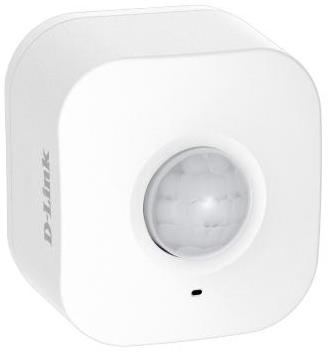
\includegraphics[width=0.4\textwidth]{images/Chapter_04/d-link-motion-sensor.jpg}
	\caption{The D-Link DCH-S150 motion sensor}
	\label{fig:d-link-motion-sensor}
\end{figure}

\subsubsection{D-Link Smart Home Devices}
OpenHAB supports the D-Link DCH-S150 (figure \ref{fig:d-link-motion-sensor}), a WiFi motion sensor.\\~\\
Pros:
\begin{itemize}
	\item Easy to install and very useful for a smart home, no special configuration needed
	\item Communication via API (OpenHAB binding)
\end{itemize}

\subsubsection{EnOcean Sensor Solutions}
EnOcean provides reliable and self-powered wireless sensor solutions for the Internet of Things. This binding allows openHAB
to monitor and control EnOcean devices through the EnOcean USB 300 gateway. EnOncean sensors include rocker switches,
environment sensors and contact sensors.\\~\\
What to consider:
\begin{itemize}
	\item We need a USB300 stick to control EnOcean devices
\end{itemize}
Pros:
\begin{itemize}
	\item Variety of sensors available
	\item Can work together with many other devices
	\item Communication via API (OpenHAB binding)
\end{itemize}
Cons:
\begin{itemize}
	\item We must have extra hardware to make them work with our system (USB 300 gateway)
\end{itemize}

\subsubsection{X10}
X10 is a company that makes gadgets like cameras and sensors for a Smart Home. This binding makes it possible to control X10 
devices via a server running the Mochad X10 daemon. Mochad is a Linux TCP gateway daemon for the X10 CM15A RF (radio frequency)
and PL (power line) controller and the CM19A RF controller. With the current version of the binding items of type Switch, Dimmer, and 
Rollershutter can be controlled. The binding only uses one-way communication so no status reading\\~\\
Pros:
\begin{itemize}
	\item Relatively low price
	\item Communication via API (OpenHAB binding)
\end{itemize}
Cons:
\begin{itemize}
	\item Low availability in Europe, mainly via specialised shops
	\item Needs extra software
	\item Offers less control than other devices
\end{itemize}

\subsection{Smart TV}

\subsubsection{LG TV}
This binding supports LG TV models with Netcast 3.0 and Netcast 4.0 (Model years 2012 and 2013), and with LG TVs which support the
UDAP 2.0 protocol over Ethernet.\\~\\
Pros:
\begin{itemize}
	\item LG Smart TVs are a very common device that should be supported by our system
	\item Communication via API (OpenHAB binding)
\end{itemize}
Cons:
\begin{itemize}
	\item OpenHAB documentation is not very specific about this binding
	\item It does not appear to support more modern LG televisions
\end{itemize}

\subsubsection{Panasonic TV}
This binding supports Panasonic TVs. It should be compatible with most up-to-date Panasonic Smart-TVs.\\~\\
Pros:
\begin{itemize}
	\item It is possible to control the TV completely from the system
	\item Panasonic TVs are a very common device
	\item Easy configuration
	\item Communication via API (OpenHAB binding)
\end{itemize}

\subsubsection{Samsung TV}
This binding integrates the Samsung TV’s.\\~\\
What to consider:
\begin{itemize}
	\item Samsung TV C (2010), D (2011), E (2012) and F (2013) models should be supported. Because Samsung does not publish any
	documentation about the TV’s UPnP interface, there could be differences between different TV models, which could lead to mismatch
	problems.
\end{itemize}
Pros:
\begin{itemize}
	\item Support for Samsung TVs is truly necessary, as they are one of the biggest Smart TV resellers
\end{itemize}
Cons:
\begin{itemize}
	\item Very limited control of the TV
	\item It has not been tested much, so we really do not have many information about this binding and if it will work with other models
\end{itemize}

\subsection{Temperature Control}

\begin{figure}
	\centering
	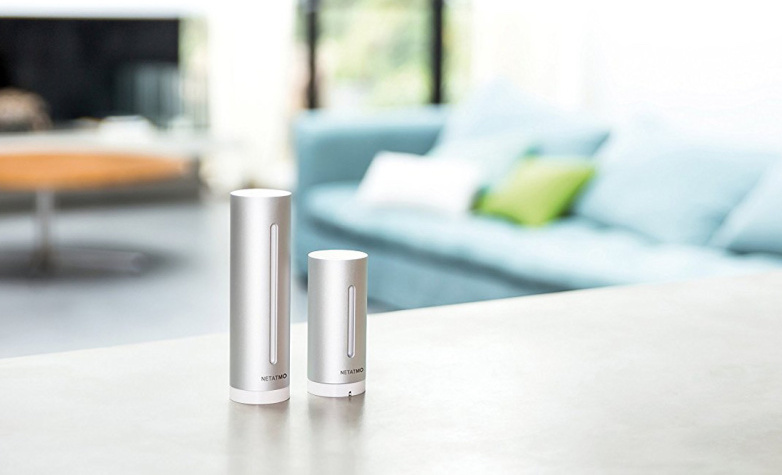
\includegraphics[width=1\textwidth]{images/Chapter_04/netatmo-weather-station.jpg}
	\caption{The Netatmo Personal Weather Station}
	\label{fig:netatmo-weather-station}
\end{figure}

\subsubsection{Devices using eBUS protocol}
The eBUS binding allows controlling the heating system. The eBUS protocol is used by heating system vendors like Wolf, Vaillant,
Kromschröder etc. It is possible to read temperatures, pump performance, gas consumption etc.\\~\\
Pros:
\begin{itemize}
	\item One of the main purposes of this Smart Home Controller is covering heating devices, thanks to this binding it is possible.
	\item Communication via API (OpenHAB binding)
\end{itemize}
Cons:
\begin{itemize}
	\item Quite complex to implement 
\end{itemize}

\subsubsection{EcoTouch Binding}
The openHAB EcoTouch binding allows interaction with Waterkotte EcoTouch heat pumps.\\~\\
Pros:
\begin{itemize}
	\item Communication via API (OpenHAB binding)
\end{itemize}

\subsubsection{MAX! Thermostats}
This is the binding for the eQ-3 MAX! Home Solution. This binding allows you to integrate, view and control the MAX! Thermostats 
in the openHAB environment.\\~\\
What to consider:
\begin{itemize}
	\item Discovery: when the Cube is found, it will become available in the discovery Inbox. Periodically the network is queried again
	for a Cube. Once the Cube is available in openHAB, all the devices connected to it are discovered and added to the discovery inbox.
	No scan is needed to trigger this.
\end{itemize}
Pros:
\begin{itemize}
	\item Communication via API (OpenHAB binding)
	\item Useful and multipurpose. For example, it is possible to track the temperature of the heating devices anytime 
\end{itemize}
Cons:
\begin{itemize}
	\item Extra device needed: MAX! Cube. It is also possible to communicate with these devices using a CUL USB Dongle rather than
	the MAX! Cube.
\end{itemize}

\subsubsection{Netatmo}
The Netatmo binding integrates the following Netatmo products:
\begin{itemize}
	\item Personal Weather Station (figure \ref{fig:netatmo-weather-station}): reports temperature, humidity, air pressure, carbon 
	dioxide concentration in the air, as well as the ambient noise level.
	\item Thermostat: reports ambient temperature, allow to check target temperature, consult and change furnace heating status....
\end{itemize}
What to consider:
\begin{itemize}
	\item Discovery: Netatmo Binding is able to discover automatically all depending modules and devices from Netatmo website. It is 
	also possible to add manually devices by creating things in in the *.things file.
\end{itemize}
Pros:
\begin{itemize}
	\item Good-looking and easy to install solutions for temperature control and temperature information
	\item Communication via API (OpenHAB binding)
\end{itemize}
Cons:
\begin{itemize}
	\item Too expensive for our price range (EUR 179 for the thermostat and EUR 169 for the weather station)
\end{itemize}

\subsection{WiFi Sockets}

\subsubsection{Orvibo S20}
This binding integrates Orvibo devices that communicate using UDP. Only supports Orvibo S20 WiFi sockets.\\~\\
Pros:
\begin{itemize}
	\item Smart Plugs enable controlling and automating non-smart devices from the controller
	\item Orvibo offers unexpensive and easy devices for this matter
	\item Communication via API (OpenHAB binding)
\end{itemize}

\subsection{Xiaomi Mi Smart Home}

This binding allows openHAB to communicate with the Xiaomi Smart Home Suite. This includes the following devices:
\begin{itemize}
	\item Xiaomi Smart Gateway v2 (with radio support)
	\item Xiaomi Smart Temperature and Humidity Sensor (round one)
	\item Xiaomi Smart Door/Window Sensor (round one)
	\item Xiaomi Wireless Switch (round one)
	\item Xiaomi Motion Sensor / IR Human Body sensor
	\item Xiaomi Smart Plug
	\item Xiaomi Smart Magic Cube
	\item Xiaomi Aqara ZigBee Wired Wall Switch (1 and 2 buttons)
	\item Xiaomi Aqara ZigBee Wireless Wall Switch (1 and 2 buttons)
	\item Xiaomi Aqara Smart Curtain
	\item Xiaomi Aqara Water Leak Sensor
	\item Xiaomi Aqara Wireless Switch (square one)
	\item Xiaomi Aqara Temperature, Humidity and Pressure Sensor (square one)
	\item Xiaomi Aqara Door/Window Sensor (square one)
	\item Xiaomi Aqara Motion Sensor (with light intensity support)
	\item Xiaomi Mijia Honeywell Gas Alarm Detector
	\item Xiaomi Mijia Honeywell Fire Alarm Detector
\end{itemize}
What to consider:
\begin{itemize}
	\item The MiHome app is necessary in order to connect the Gateway
\end{itemize}
Pros:
\begin{itemize}
	\item Xiaomi is an extremely affordable brand that offers many devices for Home Automation. 
	\item Easy to install and configure
	\item Communication via API (OpenHAB binding)
\end{itemize}
Cons:
\begin{itemize}
	\item Needs extra hardware (Smart Gateway) and software (MiHome app)
\end{itemize}

\subsection{Other devices and services}

\subsubsection{Logitech Harmony  Hub}
The Harmony Hub binding is used to enable communication between openHAB2 and multiple Logitech Harmony Hub devices. Logitech Smart
Hub devices can control other devices like Apple TV, Amazon Alexa, or Sonos devices. The Binding works as a bridge between the Harmony 
Hub and the devices connected to it.\\~\\
Pros:
\begin{itemize}
	\item Might be beneficial to consider it given the fact that there could be devices (with proprietary communication protocols) that 
	we wouldn’t be able to support, like Apple TV
	\item Communication via API (OpenHAB binding)
\end{itemize}
Cons:
\begin{itemize}
	\item Limited API
\end{itemize}

\subsubsection{Epson Projectors}
This binding is compatible with Epson projectors which support ESC/VP21 protocol over serial port.\\~\\
Pros:
\begin{itemize}
	\item Communication via API (OpenHAB binding)
\end{itemize}
Cons:
\begin{itemize}
	\item Seems that only business-oriented projectors are compatible with this binding
\end{itemize}

\subsubsection{MQTT}
This binding allows openHAB to act as an MQTT (MQ Telemetry Transport) client, so that openHAB items can send and receive MQTT 
messages from or to an MQTT broker.\\~\\
What to consider:
\begin{itemize}
	\item Implementing MQTT makes us able to use OwnTracks, a location service that uses MQTT that focuses on privacy.
\end{itemize}

\subsubsection{NTP}
The NTP binding is used for displaying the local date and time based update from an NTP server. Discovery is used to place one default 
tem in the inbox as a convenient way to add a Thing for the local time.

\subsubsection{Weather Binding}
The Weather binding collects current and forecast weather data from different providers with a free weather API. You can also display
weather data with highly customizable HTML layouts and icons. It is also possible to install the WeatherUnderground and YahooWeather
bindings.

\bigskip
\section{Voice Assistants}
The objective of this section is to explore the main voice assistants available commercially. As I explained previously, the services
provided by virtual assistants, and in particular voice assistants, are very varied. One of them is smart home control, and many of
the home-oriented voice assistants provide it. The focus on this section will be on them, the most closely related to my project.

\subsection{Samsung Bixby}
Bixby is the virtual assistant that Samsung includes in their phones, introduced in 2017, along with the introduction of the Samsung
Galaxy S8 phone. It is the evolution of their previous voice assistant, \textit{S Voice}.

Bixby is divided in three parts: \textit{Bixby Voice}, which is the voice assistant, \textit{Bixby Vision}, an assistant that works through
image recognition, and \textit{Bixby Home}, a dashboard that provides different information depending on the current
conditions.\cite{samsungBixby}

Bixby has been widely criticized for his intrusiveness and its lack of utility in many situations. In addition, it is only available in English
and Chinese at this moment. As for home automation, it is seamlessly integrated with Samsung SmartThings, making it possible to send
basic commands to devices via voice.

\subsection{Google Assistant}
Google Assistant is the name of the virtual assistant developed by Google. It was introduced in 2016, and at this moment it is
available for mobile phones (with Android and iOS operating systems), laptops, TVs, cars and smart watches. It is also integrated in
Google Home, their smart speaker.\cite{googleAssistant}

The most remarkable feature of this assistant is its ability to engage in two-way conversations, thanks to a powerful artificial intelligence
developed by Google, and Google Duplex, a new technology that Google is developing, which will allow it to have natural conversations,
mimicking the human voice.

Google Assistant is able to manage a wides range of smart home devices and in a very flexible way, thanks to its outstanding voice
recognition.

\subsection{Apple Siri}
Siri is the voice assistant developed by Apple, and the one who began the revolution of voice assistance in mobile phones. Introduced
back in 2011 and included in the iPhone 4S, it has been present in all the iOS devices (iPhones, iPads and iPods) since then, and lately
in the macOS devices (Macintosh computers) and in the Apple Watch as well.\cite{appleIOSSiri} Its range of functionalities is also
similar to its competitors, but with a slightly narrower range of possible interactions, which can make Siri feel a little less natural.

In later iOS versions, Apple has implemented Siri suggestions, which use the artificial intelligence that Siri provides to suggest
applications to the user based in the current circumstances. Siri is able to adapt over time to the user's personal preferences by
customizing search results and other responses. In the latest version of iOS, iOS 11, Siri has a much more natural voice, that can
also simulate different moods.

\subsection{Amazon Alexa}
Alexa is the virtual assistant by Amazon, and it is included by default in all their Echo devices (Amazon's smart speakers), Fire TVs
(digital media players) and Fire tablets. It is also available for iOS and Android devices as a standalone application. Its capabilities are
very similar to those of its competitors: music playback, making to-do lists, setting alarms, playing podcasts and audiobooks, providing
information, such as weather forecast and general knowledge, and of course voice interaction and home automation management.
This means that, as in the previous cases, there is also a home automation system underlying the assistant in Alexa.

Alexa differentiates from the rest on its skill system. A \textit{skill} is a functionality developed by a third-party vendor that the user
can install in the assistant in order to extend is capabilities. They can be, for instance, news services or little games. Amazon is
constantly encouraging the creation of new skills for Alexa between the developer community.\cite{amazonAlexa}

\subsection{Mycroft}
Mycroft is the name of a suite of software and hardware tools that use natural language processing and machine learning to provide
an open source voice assistant.\cite{mycroftDocumentation} Unlike the other virtual assistant we have seen previously, Mycroft is
fully open source and free. It has been undergoing heavy development since late 2017, but now it claims to be usable effectively
by developers and enthusiasts, making it the world's first fully open source AI voice assistant. But unfortunately, it is not yet usable
by the general user, as it still requires technical skills.

Mycroft is available for Linux-based operating systems and Android, but it is not ready yet for macOS and Windows, making it harder
to spread as quickly as other virtual assistants have done. However, to make up for this, they are selling their own smart speaker,
called Mark, currently in its second version.

Mycroft is modular, which makes the system easily customizable, and uses a skill system similar to Amazon Alexa. It comes with a
number of default skills, such as setting an alarm, providing the weather, or telling the time. The other skills are also installable via
voice commands, based on a list of community-contributed skills. The number of additional skills is not as high as in Alexa, but it
is constantly growing, and Mycroft encourages its users to contribute to the project.

\bigskip
The table \ref{table:voice-assistants-comparison} shows a comparison between the most important aspects of the previous voice
assistants. In this table, note that \textit{Smart Home} means having Home Automation capabilities, and always on means that the
user is able to trigger the assistant via the voice. For example, Siri is able to react to the sentence \textit{Hey Siri!}, even if the
device is with the screen off.

\begin{table}[]
	\begin{center}
		\resizebox{\textwidth}{!}{
		\begin{tabular}{|l|l|p{0.08\linewidth}|p{0.09\linewidth}|p{0.18\linewidth}|l|l|p{0.1\linewidth}|}
			\hline
			\textbf{Name} & \textbf{Developer}                                                          & \textbf{Free} & \textbf{Open source} & \textbf{Home Automation}                                    & \textbf{Mobile app}                                            & \textbf{Extra devices}                                                              & \textbf{Always on} \\ \hline
			Bixby         & Samsung                                                                     & No            & No                   & \begin{tabular}[l]{@{}l@{}}Yes\\- SmartThings\end{tabular} & \begin{tabular}[l]{@{}l@{}}Yes\\ Samsung phones\end{tabular} & No                                                                                  & Yes                \\ \hline
			Assistant     & Google                                                                      & No            & No                   & Yes                                                         & \begin{tabular}[l]{@{}l@{}}Yes\\ Android\end{tabular}        & Google Home                                                                         & Yes                \\ \hline
			Siri          & Apple                                                                       & No            & No                   & \begin{tabular}[l]{@{}l@{}}Yes\\- HomeKit\end{tabular}     & \begin{tabular}[l]{@{}l@{}}Yes\\ iOS\end{tabular}            & HomePod                                                                             & Yes                \\ \hline
			Alexa         & Amazon                                                                      & No            & No                   & Yes                                                         & \begin{tabular}[l]{@{}l@{}}Yes\\ iOS, Android\end{tabular}   & \begin{tabular}[l]{@{}l@{}}Echo\\ Echo Dot\\ Echo Dot Kids\\ Echo Plus\end{tabular} & Yes                \\ \hline
			Mycroft       & \begin{tabular}[l]{@{}l@{}}Mycroft and the\\ Mycroft Community\end{tabular} & Yes           & Yes                  & Yes                                                         & \begin{tabular}[l]{@{}l@{}}Yes\\ Android\end{tabular}        & \begin{tabular}[l]{@{}l@{}}Mark II\\ Mark I\end{tabular}                            & Yes                \\ \hline
		\end{tabular}}
	\caption{Comparison between different voice assistants}
	\label{table:voice-assistants-comparison}
	\end{center}
\end{table}
